\chapter{实现}
\label{chp:implementation}

\par 在第~\ref{chp:cw-cache}章中我们对问题进行了建模并且对我们提出的Bundle-K的方案做了理论分析,论证了我们的方案的可行性。在本章当中我们会介绍CW-Cache的具体实现。

\section{架构概览}
\label{sec:archi-overview}

\par 我们在~\ref{subsec:alluxio}小节中介绍过的分布式内存文件系统Alluxio上实现了CW-Cache,图~\ref{fig:cw-cache-archi}展示了CW-Cache的整体框架。CW-Cache系统主要由两部分组成:CW-Master和CW-Client,它们分别是在Alluxio Master和Alluxio Client的基础上实现的。

\par CW-Master实现了第\ref{chp:cw-cache}章中描述的Bundle-K方案的主要逻辑,除了原来Alluxio Master具有的响应Client的请求、维护全局的文件的元数据之外,还要记录保存查询任务对数据表中列的访问次数,运行Bundle-K方案中的逻辑对数据表进行列级别的复制,当Client访问数据表中的列的时候返回所有副本所在位置。

\par CW-Client依旧是用户的应用与系统交互的桥梁。CW-Cache接受应用的读/写请求,并与CW-Master交互获得文件所在位置,在执行SQL查询任务的时候,CW-Client会发起远程调用,上传访问的文件的URI、偏移量(Offset)和长度。读取数据表的列所在的文件时,它收到CW-Master传来的副本(原表)所在的位置,根据一定的策略自行决定从哪里读取。此外,图中的应用主要指上层应用框架,比如Spark,Hive等等,通过Alluxio提供的通用接口存取文件。Cache Server上由Alluxio Worker来管理本地节点的文件或者对象。

\begin{figure}[]
	\centering
	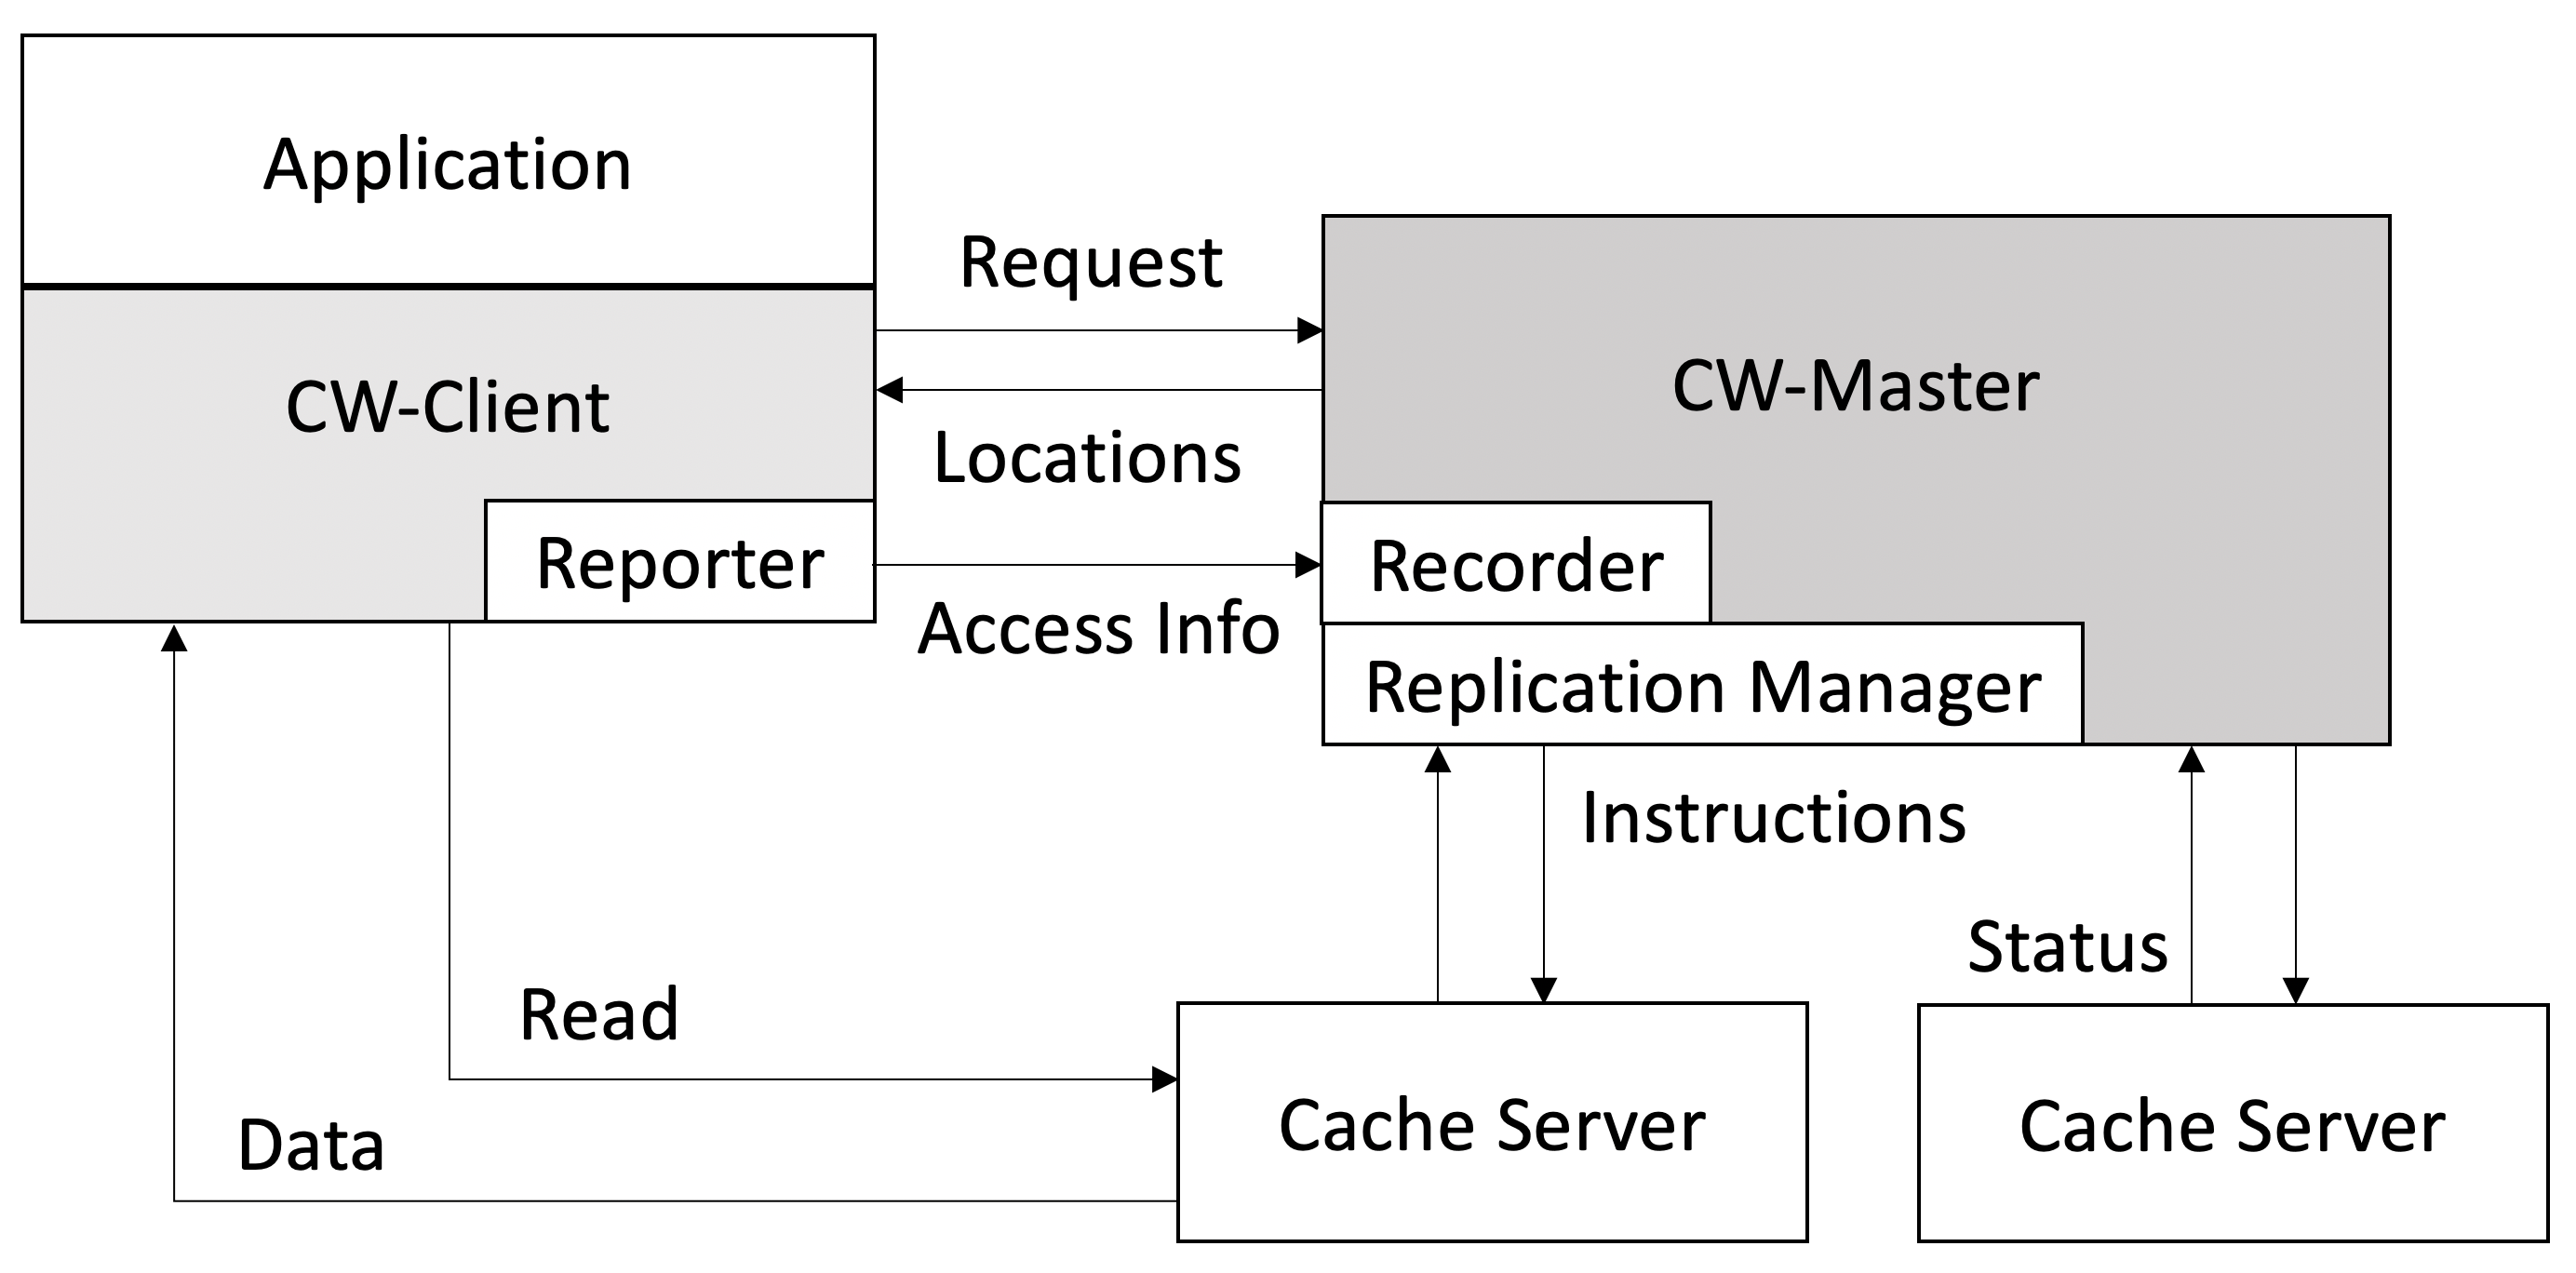
\includegraphics[width=0.8\textwidth]{img/implementation/cw-cache-archi}
	
	\caption{简单方案的架构设计。}
	\label{fig:cw-cache-archi}
	%\vspace{-.1in}
\end{figure}

\par Reporter是增加在Client端用于将应用访问的文件的信息:文件URI,偏移量和长度汇报给Master;Recorder是在Master端用于接收Reporter汇报的数据并将其存储在特定的数据结构中,维护热度的统计信息;Replication Manager负责利用数据表的列的热度数据,执行第~\ref{chp:cw-cache}章中的Bundle-K方案,计算出$K$和复制的份数$r$,对前$K$个最热门列进行“捆绑”复制。此外,Replication Manager也会在CW-Client的读请求到来时返回所有副本(如果有)的位置,供其选择。

\section{实现细节分析}
\label{sec:impl-details}

\par 在本节中我们会介绍CW-Cache系统实现的细节,介绍我们在alluxio之上添加的部分代码,以及一些注意事项。

\subsection{Reporter}

\par Reporter的功能是将读取文件的信息:文件URI、偏移量、读取长度,上传给CW-Master。第~\ref{chp:column-aware}章提到的简单方案是需要上层应用提供访问的列的语义信息,也就是使得CW-Cache得知应用具体访问的列。在~\ref{subsec:simp-analysis}小节我们提到,我们放弃采用这种方法,是因为它需要上层计算框架与中间层的耦合,不符合软件设计模块化、低耦合的原则。我们想要在中间层实现列级别的负载均衡,利用尽可能少的信息,而Alluxio原本提供的读文件的接口就是接受文件URI、偏移量、读取长度这三个参数。所以,为了方便代码实现,减少代码的耦合度,我们放弃了让上层将Parquet文件的语义信息传给Alluxio的想法,转为利用这三个参数构成的更加底层的信息,我们将之称为“文件片段”。Alluxio Client在读取文件的时候,只是将文件URI通过远程调用传给Master,Master返回文件所在的workers,Client去相应的worker找到文件,根据偏移量和读取长度读取应用需要的部分,也就是说,偏移量和读取长度仅Client可见。为了实现这个Reporter,我们添加了一个远程调用,将这三样信息一起传给Master。Alluxio 1.8.0版本使用Apache Thrift作为远程调用框架,我们在定义接口的thrift文件里定义:

\begin{lstlisting}[language=c]
struct UploadFileSegmentsAccessInfoTResponse{
  1: list<fileSegmentInfo> replList
}
/**
* Upload UFSPath, offset and length to master for recording.
*/
UploadFileSegmentsAccessInfoTResponse uploadFileSegmentsAccessInfo(
  /** the UFSPath of the file*/ 1: string UFSPath,
  /** the offset in the file*/ 2: i64 offset,
  /** the length of bytes to be read*/ 3: i64 len,
) throws (1: exception.AlluxioTException e)
\end{lstlisting}


\subsection{Recorder}
\label{subsec:impl-recorder}

\par Recorder用于记录应用访问的列的信息,它实质是Replication Manager的一部分,我们把它作为Replication Manager的一个方法:

\begin{lstlisting}[language=java]
  public Map<AlluxioURI, OffLenPair> recordAccess(AlluxioURI requestFile, long offset, long length);
\end{lstlisting}

\par 这个方法传入了之前提到的文件URI、偏移量和读取长度三个参数,返回的是文件URI和偏移量、读取长度组成的配对的映射,这是因为这个方法是Reporter远程调用在Master端的实现,该远程调用也需要返回读取的文件片段的副本,以供Client选择。为了存储文件的访问信息,我们设计了\verb|FileAccessInfo| 类,它的成员变量和主要成员函数如下:

\begin{lstlisting}[language=java]
public class FileAccessInfo {
  private AlluxioURI mFilePath;
  private Map<OffLenPair, Long> offsetCount;
  private long queryNum;
  private long lastAccessTime; /* estimate query based on interval */
  private long recordInterval;
  private Set<OffLenPair> offsetWithinQuery;

  public void incCount(OffLenPair offLenPair){
    offsetCount.merge(offLenPair, (long) 1, Long::sum);
    long currentTime = CommonUtils.getCurrentMs();

    // check if it belongs to a new query
    if (currentTime - lastAccessTime > recordInterval){
      queryNum++;
      offsetWithinQuery.clear();
    }
    else {
      if (offsetWithinQuery.contains(offLenPair)){
        queryNum++;
        offsetWithinQuery.clear();
      }
      else {
        offsetWithinQuery.add(offLenPair);
      }
    }

    lastAccessTime = currentTime;
  }
  ...
}
\end{lstlisting}

\par 根据~\ref{sec:estimate-patern}节,对于一张数据表(即\verb|mFilePath| 标识)来说,用列的热度来估算共同访问模式,需要得到访问过这张表的查询任务的数量,在代码里对应成员变量queryNum,以及每个列的访问次数,因为实现中用底层文件代替具有语义信息的列,因此代码里是\verb|Map<OffLenPair, Long> offsetCount| 来记录。成员函数\verb|public void incCount(OffLenPair offLenPair)| 是用于增加计数的,代码里引入\verb|lastAccessTime| 和 \verb|recordInterval| ,是因为我们在上传信息的时候没有附带Client的身份标识,这样Master对所有的请求一视同仁,所以我们设置时间窗口来近似估计哪些文件读取请求来自同一个查询任务。这样做的前提是我们认为同一个查询任务访问不同列的时间间隔很短,当然在多用户使用系统的情况下,得出的数据会损失部分准确性。

\subsection{Replication Manager}

\par Replication Manager根据Recorder记录的统计信息,运行第~\ref{chp:cw-cache}章中描述的关于Bundle-K方案中的算法,决定$K$和复制数量$r$, 是CW-Cache系统的核心部分,并将需要复制的部分取出作为新的文件缓存在集群中。为此,我们在原Alluxio Master模块中添加了\verb|repl| 模块,其核心是\verb|ReplManager| 类。在~\ref{subsec:impl-recorder}小节中描述的Recorder实际是属于这个类的,这个类的成员变量主要有:

\begin{lstlisting}[language=java]
private FRClient frClient;
private ReplPolicy replPolicy;
private Map<AlluxioURI, FileAccessInfo> accessRecords;
private Map<AlluxioURI, FileRepInfo> fileReplicas;
private Map<AlluxioURI, AlluxioURI> replicaMap;
private Map<AlluxioURI, FileOffsetInfo> offsetInfoMap;
private int checkInterval; /* in seconds */
\end{lstlisting}

\par 其中,\verb|accessRecords| 是Recorder的实例;\verb|fileReplicas| 、\verb|replicaMap| 、\verb|offsetInfoMap|是用于复制;\verb|replPolicy|是复制策略的接口,目前我们的实现是Bundle-K,Bundle-K的代码见附录~\ref{appendix:bundle-k-code},后续我们会针对Bundle-K方案的不足之处开发新的策略,以及一些更加基础、简单的策略来和Bundle-K进行对比;\verb|frClient|是我们添加的一个特殊的Client,它专门用于Master在对文件进行复制的时候,能够像普通的Client一样调用文件系统的功能来完成副本的复制、删除等操作。

\subsection{周期性检查与复制}

\par 因为数据表的各个列的热度可能随着时间的推移而改变,CW-Cache通过对缓存的数据表\emph{重新复制}来使缓存服务器\emph{周期性地负载均衡}。沿用论文~\cite{ananthanarayanan2011scarlett}中推荐的方法,CW-Cache每$12$小时基于过去$24$小时记录的各数据表的各个列的访问计数对文件重新重新复制。为了达到这个目的,\texttt{CW-Master} 在平常时间会持续对各个列的访问进行记录,同时它注册一项服务,每隔$12$小时调用Replication Manager的\texttt{checkStats()} 成员函数,master用章节~\ref{chp:cw-cache}描述的方法估算列的共同访问模式,进一步计算最佳的要复制的列的数量 $K$和复制的份数$r$。本身CW-Cache系统里缓存有原表和副本,我们只需要执行Bundle-K的方案计算新的$K$和$r$,如果$K$和$r$没有发生变化,那么什么都不用做;如果仅仅$K$改变,那么就通过复制或者删除副本使副本数量为$r$;如果两者均发生改变,那么就删除所有副本,重新复制即可。

\par 我们有证据来支持周期性进行这个过程的有效性:在短期内(比如一天)生产集群中的文件热门程度是\emph{相对稳定}的。事实上,研究人员观察到,在一个Microsoft的集群中,任何一天中被访问到的$40\%$的文件,在之前与之后的四天里同样被访问~\cite{ananthanarayanan2011scarlett}。一个类似的结论也可以从Yahoo! 集群数据集~\cite{yahoo!_trace}中得到:接近$27\%$的文件保持超过一周的热门程度。


\section{系统额外开销}

\par 元数据的存储开销。为了统计文件片段的热度信息,Master需要在内存中维持一部分元数据。对于每一个Parquet文件(可以是某一个Parquet文件的一部分)来说,CW-Cache Master要维护它被访问过的文件片段(由偏移量和读取长度构成)的计数器,以及原文件片段和复制过后的文件片段(可能是多个)的映射。这部分元数据,我们仅保留一段时间的,而不是历史累加,毕竟访问模式一直在变化,目前实现中是12小时复制分发一次,那么这些元数据就维护12小时,之后便重新统计。相对于Alluxio本身维护的文件的元数据来说,这些开销是很小的。

\par 计算开销。求出复制的列的数量$K$和复制的份数$r$的这个过程是我们的系统实现中的主要开销。第~\ref{sec:alg}节的理论表明,算法的时间内复杂度是$O(m\log{m} + n)$,$m$是访问模式的数量,$n$是列的数量,整个过程中也采用了不少近似处理,计算并不复杂。这个计算在目前的实现中是12小时进行一次,并且我们可以根据经验把这个时间设置为类似深夜这样的少有人使用系统的时间,这样的话计算开销的影响就极小了。
